%\documentclass[svgnames,dvipsnames,usenames]{beamer}		        % version standard
\documentclass[svgnames,dvipsnames,usenames,handout]{beamer}        % version imprimable pour assistance
%\documentclass[svgnames,dvipsnames,usenames,notes=show]{beamer}    % version imprimable avec notes d’orateur
%\documentclass[svgnames,dvipsnames,usenames,notes=only]{beamer}    % version imprimable avec notes d’orateur

\usepackage[utf8]{inputenc}
\usepackage[frenchb]{babel}
\usepackage{graphicx}	% pour insérer des figures
\usepackage{ruby}
\usepackage{iwona} 

\usetheme{progressbar}
%\progressbaroptions{headline=none,frametitle=picture-section}
\progressbaroptions{titlepage=picture, headline=sections, frametitle=picture-section, imagename=images/markus_logo_big.png}

\logo{\includegraphics[scale=0.05]{images/logo_ECN.png}} % Logo qui sera affiché en bas à droite

\title[]{Contribution des Étudiants de l’École Centrale de Nantes à MarkUs, un projet libre}
\subtitle{}
\author[M. \textsc{Magnin}, G. \textsc{Moreau}, N. \textsc{Varoquaux}, B. \textsc{Vialle}]%
{Morgan \textsc{Magnin}, Guillaume \textsc{Moreau}, Nelle \textsc{Varoquaux} et Benjamin \textsc{Vialle}}
\institute{École Centrale de Nantes}
\date{Rencontres Mondiales du Logiciel Libre - 11/07/2011} %\today

\hypersetup{
		pdfpagemode = Fullscreen, %afficher le pdf en plein écran
		pdfauthor = Morgan Magnin, Guillaume Moreau, Nelle Varoquaux, Benjamin Vialle.
		pdftitle = Contribution des Étudiants de l’École Centrale de Nantes à MarkUs, un projet libre,
		pdfsubject = MarkUs,
		pdfkeywords = {MarkUs, Ruby, Ruby on Rails, École Centrale de Nantes, RMLL, Contribution d'étudiants à des projets libres},
		%pdfcreator = PDFLateX,
		%pdfproducer = PDFLaTeX,
}

% Pour griser les items
\beamertemplatetransparentcovered

%\usepackage{pgfpages}
%\setbeameroption{show notes on second screen=right}
%\setbeameroption{show notes on second screen=location}

\begin{document}

\frame{\titlepage}

\frame{\frametitle{Présentation}\tableofcontents} 

\section{L'Ecole Centrale de Nantes et le Libre}

\frame
{
  \frametitle{École Centrale de Nantes}

  \begin{block}{École d'ingénieur généraliste}
  Accessible principalement après les classes préparatoires, elle développe :
    \begin{itemize}[<+->]
      \item des compétences scientifiques et techniques
      \item des compétences humaines :
      \begin{itemize}
	  	\item une capacité à {\bf s'intégrer}
		\item une capacité à {\bf communiquer}
		\item une capacité à {\bf partager}
      \end{itemize}
    \end{itemize}
  \end{block}
  
  \begin{block}{Enseignement}
  	Deux ans de tronc commun, suivi d'une année de spécialisation
  \end{block}
  
  \begin{alertblock}{}
    Participation d'étudiants de troisième année option informatique à des projets libres, pour ceux qui le souhaitent.
  \end{alertblock}
}

\frame{
  \frametitle{En parallèle, un besoin...}
  {\bf Comment gérer et évaluer efficacement les travaux des étudiants en
  TP/Projet ?}
  \begin{itemize}[<+->]
    \item Enseignants
    \begin{itemize}
      \item Gros volume de soumissions à traiter (plusieurs centaines par TP)
      \item Problématique d'harmonisation des notes entre groupes et correcteur
      \item Retour des corrections aux étudiants
    \end{itemize}
    \item Etudiants
    \begin{itemize}
      \item Comment récupérer les TP corrigés ?
    \end{itemize}
  \end{itemize}
}

\frame{
  \frametitle{Le workflow actuel}
  \includegraphics[scale=0.50]{images/WF-projet-avant.png}
  \begin{center}
  \end{center}
}


\frame{
  \frametitle{Markus, un outil de correction en ligne de travaux étudiant}
  \begin{itemize}[<+->]
    \item Application Web
    \item Destiné à l'évaluation de projet informatique
    \item Dépôt versionné des travaux des étudiants
  \end{itemize}
}


\section{Markus à l'École Centrale de Nantes}
\frame{
  \begin{itemize}[<+->]
    \item 4 développeurs principaux
    \item Équipe trimestrielle d'étudiant
  \end{itemize}

  \begin{itemize}[<+->]
    \item \textit{Turnover} des developpeurs très importante
    \item Difficulté pour maintenir une équipe stable qui comprenne la
    totalité du code
    \item Projet non communautaire, dirigé par les demandes des clients
    et les projets étudiants
  \end{itemize}
}

\frame{

  \frametitle{La nécessité d'un mentor technique}

  }

\frame{
  \frametitle{Un projet étudiant type à Centrale Nantes}

  \begin{itemize}[<+->]
    \item Écriture d'un cahier des charges
    \item Implémentation de(s) fonctionnalité(s)
    \item Redaction de rapport hebdomadaire
    \item Réunion hebdomadaire avec l'encadrant
    \item Réunion hebdomadaire avec le mentor technique
    \item Rédaction d'un rapport final
    \item Présentation de 20min
  \end{itemize}
}


\frame{
\frametitle{Un projet étudiant type sur Markus}

  \begin{center}
  \includegraphics[scale=0.50]{images/markus-projet-etudiant_01.png}
  \end{center}
}

\frame{
  \frametitle{Un projet étudiant type sur Markus}
  \begin{center}
  \includegraphics[scale=0.50]{images/markus-projet-etudiant_02.png}
  \end{center}
}

\frame{
  \frametitle{Un projet étudiant type sur Markus}
  \begin{center}
  \includegraphics[scale=0.50]{images/markus-projet-etudiant_03.png}
  \end{center}
}

\frame{
  \frametitle{Un projet étudiant type sur Markus}
  \begin{center}
  \includegraphics[scale=0.50]{images/markus-projet-etudiant_04.png}
  \end{center}
}


\section{QA}
 
\frame{
  \frametitle{Assurance Qualité et suivi du code}
  
  \begin{block}{}
  \end{block}
}


\frame{
  \frametitle{Un projet étudiant type sur Markus}
  \begin{center}
  \includegraphics[scale=0.50]{images/markus-projet-etudiant_05.png}
  \end{center}
}

\frame{
  \frametitle{Difficultés rencontrées par les étudiants}
  \begin{itemize}[<+->]
    \item Projet complex:
    \begin{itemize}
      \item Rails, Ant, Git \dots
      \item 15~000 de ligne de code
      \item Présence non physique des mentors techniques
      \item Processus d'Assurance Qualité très strict
    \end{itemize}
  \end{itemize}
  
  \begin{alertblock}{}
    Il est difficile d'avoir un patch intégré à la fin du projet
  \end{alertblock}
}

\section*{Conclusion}

\frame{
  \frametitle{Conclusion}

  Listes des fonctionnalités implémentées par des étudiants ECN dans Markus:
  \begin{itemize}[<+->]
    \item Gestion des groupes - invitation des étudiants (Nelle Varoquaux)
    \item Refonte de l'interface utilisateur (Nelle Varoquaux)
    \item Framework de test (Benjamin Vialle)
    \item Implémentation des sections (Nelle Varoquaux \& Christian Jacques)
    \item Internationalisation \& traduction en français (Benjamin Vialle)
    \item Ajout d'un module d'annotation tactile (Clément delafargue, Benjamin Vialle
	  etc) \emph{en cours}
    \item Ajout d'un module d'annotation de formules mathématiques (Anthony Le
	  Jalle \& Mickael Lumbroso) \emph{en cours}
    \item Ajout d'un module de détection de plagiat (Shion Kashimura \& Benjamin
	  Thorrent) \emph{en cours}
    \item Migration à Rails 3 (Benjamin Vialle) \emph{en cours}
  \end{itemize}

}



%\bibliography{biblio}
%TODO Bibliographie
% http://eat-tice.ec-nantes.fr/wp-content/uploads/2011/06/magnin-moreau-QPES2011.pdf

%\bibliographystyle{alpha}

\end{document}
